% chapter4_srs.tex

\section{Chapter Overview}
This chapter specifies the functional and non-functional requirements of RootLens, documents stakeholder analysis, and presents the visual models that define the system boundary and interactions. Requirements were elicited through literature review, questionnaire survey, and iterative prototyping, and prioritised using the MoSCoW method.

\section{Rich Picture Diagram}
The Rich Picture Diagram in Figure~\ref{fig:rich_picture} provides an informal, high-level depiction of the problem domain. It illustrates the central Kubernetes cluster, KEDA's role in event-driven scaling, the RabbitMQ trigger, the three categories of scaling delay, and RootLens as the proposed solution feeding diagnostic results to the React dashboard consumed by SRE and DevOps engineers.

\begin{figure}[H]
\centering
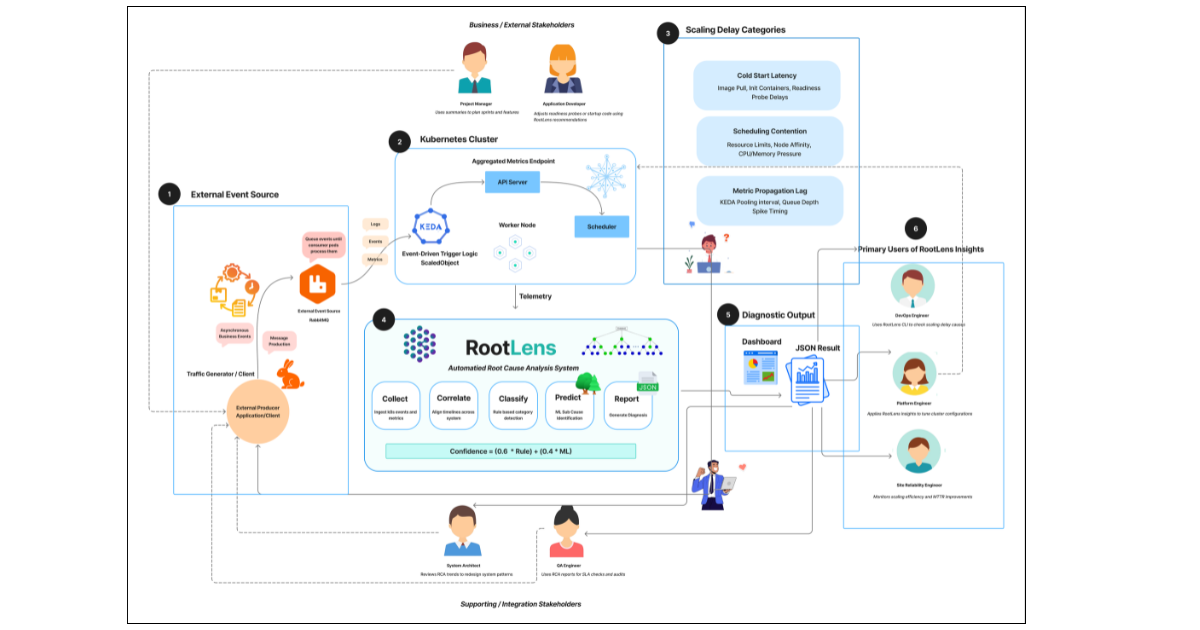
\includegraphics[width=1.0\textwidth]{thesis/assets/rich_picture_diagram.png}
\caption{Rich Picture Diagram of the RootLens Problem Domain}
\label{fig:rich_picture}
\end{figure}

\section{Stakeholder Analysis}

\subsection{Stakeholder Onion Model}
The Stakeholder Onion Model in Figure~\ref{fig:onion} maps stakeholders by proximity to the system. The innermost ring (\textbf{Core}) contains direct daily users (SRE and DevOps engineers); the middle ring (\textbf{Operational}) contains stakeholders affected by outputs but not operating the system (Platform Engineers, Engineering Managers); and the outer ring (\textbf{Institutional}) contains supervisory parties (Academic Supervisor, University).

\begin{figure}[H]
\centering
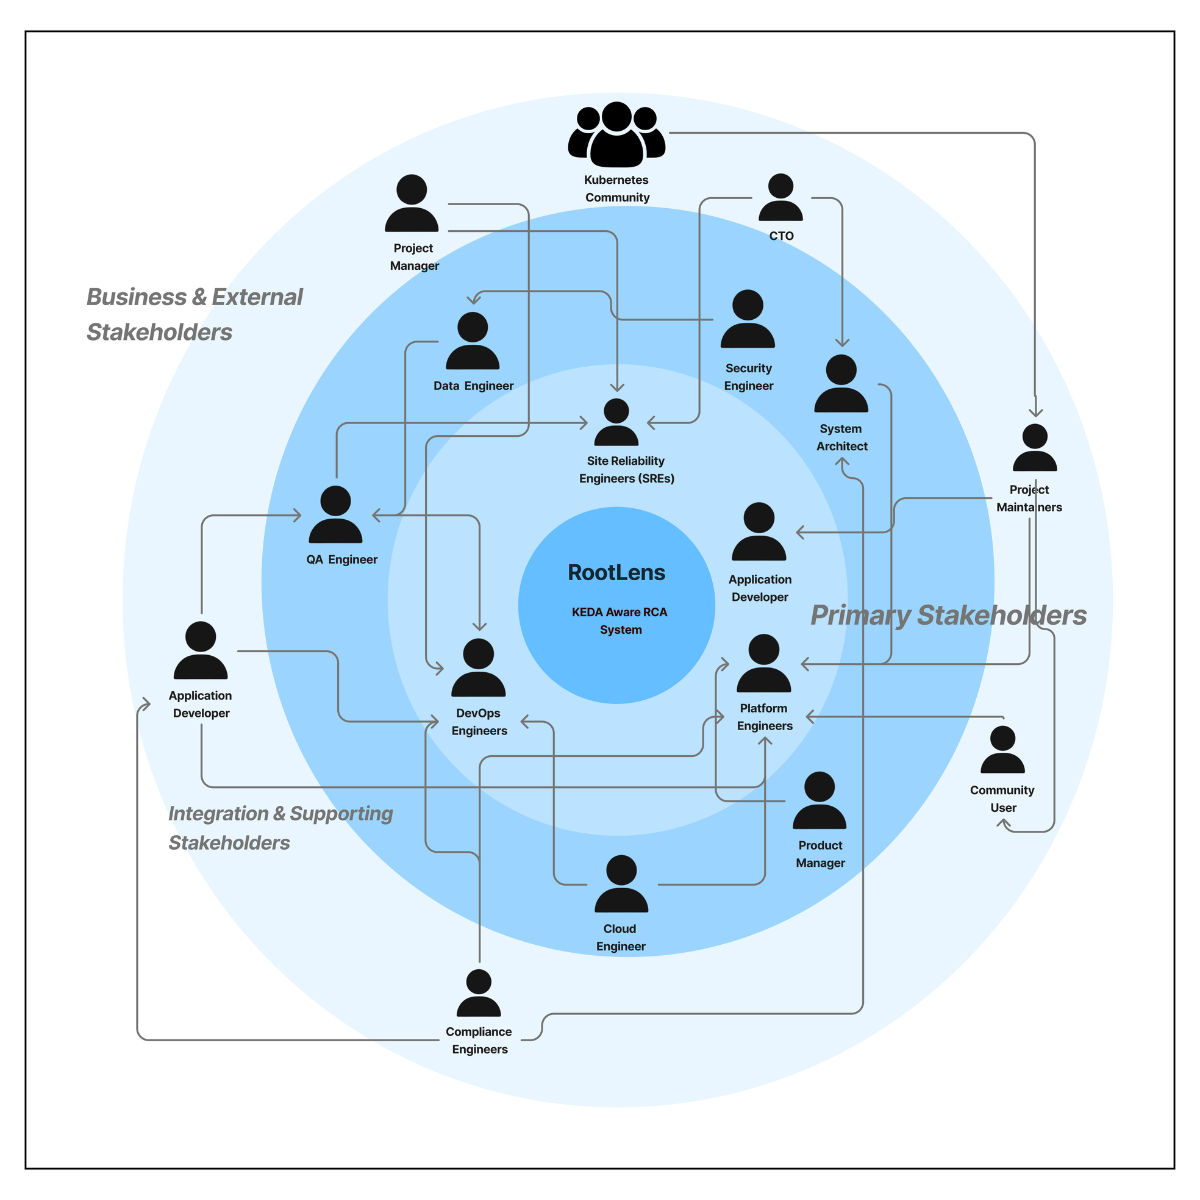
\includegraphics[width=1.0\textwidth]{thesis/assets/stakeholder_onion_diagram.png}
\caption{Stakeholder Onion Model for RootLens}
\label{fig:onion}
\end{figure}

\subsection{Stakeholder Viewpoints}
Table~\ref{tab:stakeholder_viewpoints} documents the expectations and needs of each stakeholder group identified in the onion model.

\begin{xltabular}{\textwidth}{|p{2cm}|p{2.5cm}|X|p{4cm}|}

\hline
\textbf{Ring} & \textbf{Stakeholder} & \textbf{Viewpoint / Expectations} & \textbf{Key Requirements} \\ \hline
\endfirsthead

\hline
\textbf{Ring} & \textbf{Stakeholder} & \textbf{Viewpoint / Expectations} & \textbf{Key Requirements} \\ \hline
\endhead

Core & SREs & Primary daily users; need fast, accurate diagnosis of scaling delays to reduce MTTD and prioritise investigation via confidence scores. & FR03, FR04, FR06, NFR01, NFR02 \\ \hline
Primary & DevOps Engineers & Operate clusters and respond to incidents; require actionable sub-cause output and REST API integration with existing tooling. & FR06, FR08, FR09, NFR01 \\ \hline
Primary & Platform Engineers & Maintain cluster infrastructure; need Kubernetes-native deployment and compatibility with standard orchestration. & FR10, FR15, NFR04, NFR07 \\ \hline
Primary & Application Developers & Deploy workloads affected by scaling delays; need visibility into whether delays are application-level or infrastructure-level. & FR07, FR11 \\ \hline
Primary & System Architects & Design platform reliability; require the system to follow microservice best practices and support graceful degradation. & FR13, FR14, NFR05 \\ \hline
Primary & Security Engineers & Enforce credential hygiene and secure communication across services. & NFR05, NFR06 \\ \hline
Supporting & QA / Cloud Engineers & Validate system correctness and cloud deployment; need reproducible test environments and clear API contracts. & FR14, NFR04, NFR07 \\ \hline
Supporting & Product Managers & Require visibility into scaling failure trends for capacity planning and feature prioritisation decisions. & FR09, FR10, FR12 \\ \hline
External & CTO / Project Managers & Strategic oversight; expect the tool to reduce operational costs and improve incident response times. & NFR01, NFR02 \\ \hline
External & K8s Community & Open-source consumers; expect clear documentation, standard CRD patterns, and portability across clusters. & FR15, NFR07 \\ \hline

\caption{Stakeholder Viewpoints}
\label{tab:stakeholder_viewpoints}
\end{xltabular}

\section{Selection of Requirements Elicitation Methodologies}
Three methodologies were employed to gather requirements:

\begin{itemize}
    \item \textbf{Literature Review (Archival Research):} Systematic review of 20+ papers on Kubernetes autoscaling, RCA, cold start latency, and ML-based operational systems. The primary functional requirements were identified from gaps documented in prior research.
    \item \textbf{Questionnaire Survey (Quantitative):} A structured, closed-ended online questionnaire distributed to practising DevOps and SRE professionals to gather data on diagnostic pain points, acceptable latency thresholds, and dashboard priorities. The questionnaire is provided in Appendix~A.
    \item \textbf{Prototyping (Iterative):} An early rule-based prototype tested against real Minikube scenarios to empirically calibrate timing signal thresholds and feature definitions.
\end{itemize}

\section{Discussion of Findings}

\subsection{Literature Review Findings}
Chapter~2 identified: no existing system classifies KEDA autoscaling delays (FR01, FR03); ML sub-cause classification requires real experimental data (Basiri et al., 2016); Random Forest achieves high accuracy on small Kubernetes datasets (Toka, Varga and Marosi, 2021) (FR05); and a gap exists in hybrid rule-ML RCA systems (Soldani and Brogi, 2022) (FR06).

\subsection{Survey Findings}
The questionnaire comprised 10 closed-ended questions sent to 25 practitioners, with 15 responses (60\% response rate). All respondents had at least one year of Kubernetes experience. Key findings:

\begin{itemize}
    \item 73\% encounter autoscaling delays at least monthly.
    \item 67\% report manual diagnosis takes 5-30 minutes, informing NFR01.
    \item 87\% rated confidence scores as important, informing FR06.
    \item 80\% require sub-second response time, reinforcing NFR01.
    \item Most requested dashboard features: real-time confidence (80\%), historical trends (67\%), sub-cause breakdowns (60\%).
    \item 73\% would integrate an automated RCA tool into on-call workflows.
\end{itemize}

Full survey response charts are presented in Appendix~A (Figures~\ref{fig:app_q1}-\ref{fig:app_q10}).

\subsection{Prototyping Findings}
An early prototype on Minikube identified: image pull duration ($>$30s) as the primary cold start discriminator (FR04); scheduling duration alone cannot distinguish sub-causes, confirming the need for ML (FR05); the system must degrade gracefully without ML (FR13); and the API must return both root cause and sub-cause in a single response (FR08, FR09).

\section{Summary of Findings}
Table~\ref{tab:elicitation_summary} maps key findings from each elicitation method to the requirements they informed.

\begin{xltabular}{\textwidth}{|p{2cm}|X|X|}

\hline
\textbf{Source} & \textbf{Key Finding} & \textbf{Requirement Informed} \\ \hline
\endfirsthead

\hline
\textbf{Source} & \textbf{Key Finding} & \textbf{Requirement Informed} \\ \hline
\endhead

Literature & No existing system classifies KEDA delays into the three categories & FR01: Automated detection, FR03: Three-category classification \\ \hline
Literature & ML sub-cause classification requires real experimental data & Custom fault-injection dataset (Chapter~7) \\ \hline
Literature & Random Forest effective for Kubernetes tasks with small datasets & FR05: Category-specific ML explainer models \\ \hline
Literature & Gap in hybrid rule+ML RCA systems & FR06: Weighted confidence combination \\ \hline
Survey & Manual diagnosis takes 5-30 minutes (67\% of respondents) & NFR01: Sub-300ms RCA latency \\ \hline
Survey & Confidence scores rated important by 87\% of respondents & FR06: Weighted confidence combination \\ \hline
Survey & Dashboard must show history and trends (67\% priority) & FR09: RCA history endpoint, FR12: Trend chart \\ \hline
Survey & 80\% require sub-second latency for automated RCA & NFR01: Sub-300ms RCA latency \\ \hline
Prototype & Image pull duration is the primary cold start discriminator ($>$30s threshold) & FR04: Cold start feature extraction \\ \hline
Prototype & Scheduling duration alone cannot distinguish sub-causes & FR05: ML-based sub-cause classification \\ \hline
Prototype & System must continue functioning when ML service is unavailable & FR13: Graceful degradation \\ \hline

\caption{Requirements Elicitation Summary}
\label{tab:elicitation_summary}
\end{xltabular}

\section{Context Diagram}
The Context Diagram in Figure~\ref{fig:context} depicts RootLens as the central system and its interactions with all external entities at DFD Level~0. Four external systems supply observability data (Kubernetes API, KEDA Controller, RabbitMQ Management API, Prometheus), while three external consumers receive diagnostic outputs (SRE/DevOps engineers, external monitoring tools, engineering managers). The Level~1 Data Flow Diagram in Chapter~6 is derived from this context diagram.

\begin{figure}[H]
\centering
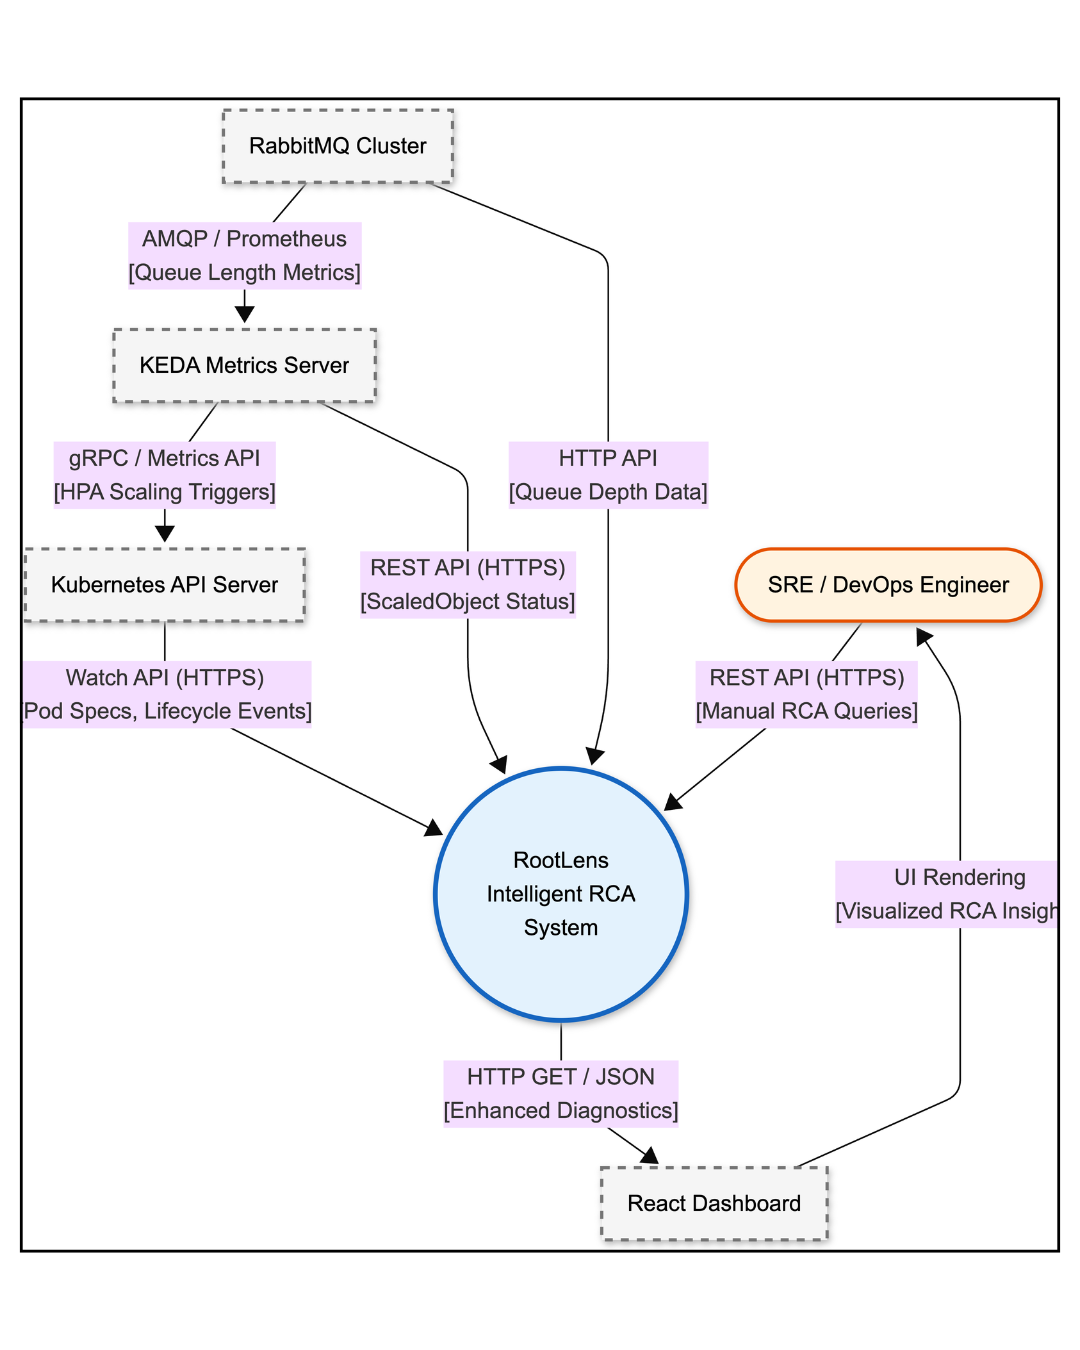
\includegraphics[width=0.85\textwidth]{thesis/assets/context_diagram.png}
\caption{Context Diagram (DFD Level~0) for RootLens}
\label{fig:context}
\end{figure}

\section{Use Case Diagram}
The Use Case Diagram in Figure~\ref{fig:usecase} shows the four primary use cases and their actors. The Kubernetes Cluster acts as an automated trigger; SRE and DevOps engineers are the primary human consumers; and External Monitoring Systems represent programmatic API consumers.

\begin{figure}[H]
\centering
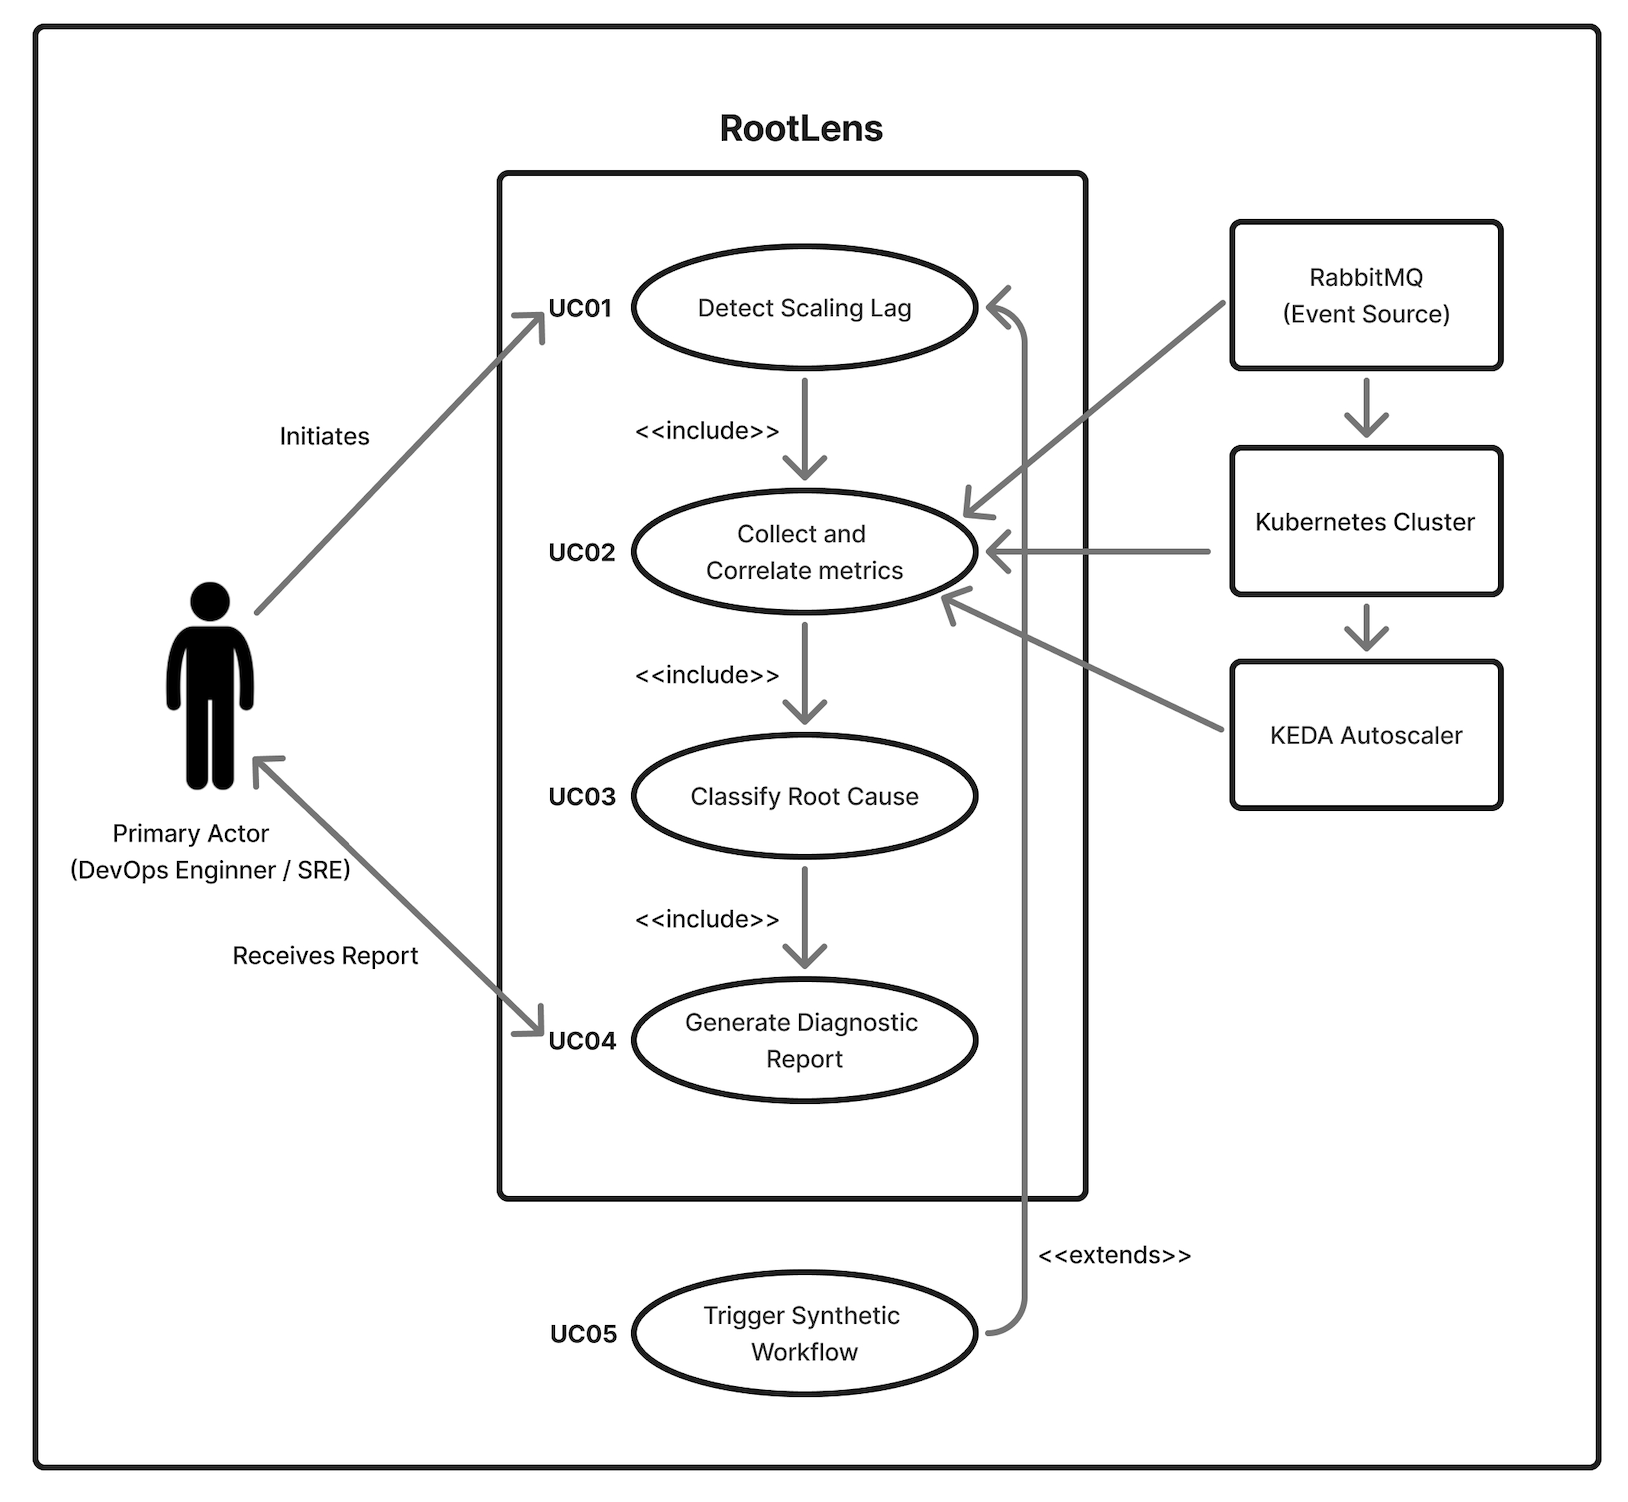
\includegraphics[width=0.85\textwidth]{thesis/assets/usecase_diagram.jpg}
\caption{Use Case Diagram Showing Primary Actors and System Use Cases}
\label{fig:usecase}
\end{figure}

\subsection{UC1: Trigger Root Cause Analysis}
\textbf{Actor:} Kubernetes cluster (automated).
When a KEDA-triggered scaling event is detected, RootLens collects timing signals, applies the rule-based classifier, invokes the ML explainer, combines confidence, and stores the result. If the ML service is unavailable, the system degrades gracefully by storing a rule-based-only result with $C_{\text{final}} = C_{\text{rule}}$.

\subsection{UC2: View RCA Dashboard}
\textbf{Actor:} SRE / DevOps Engineer.
The engineer opens the React dashboard to view the most recent RCA result, historical trends, confidence scores, and sub-cause explanations with feature importance breakdowns. If no results are stored, an empty state message is displayed.

\subsection{UC3: Query RCA API}
\textbf{Actor:} External monitoring system or SRE tool.
An external system queries the REST API to retrieve RCA results programmatically as JSON.

\subsection{UC4: View System Health}
\textbf{Actor:} DevOps Engineer.
The engineer queries the health check endpoint to verify component status. If the ML service is unreachable, the system reports as degraded.

\section{Requirements}

\subsection{MoSCoW Prioritisation}
Requirements were prioritised using the MoSCoW method: \textbf{Must Have} (M) requirements are mandatory; \textbf{Should Have} (S) are important and expected; \textbf{Could Have} (C) are desirable enhancements; \textbf{Won't Have} (W) are explicitly out of scope.

\subsection{Functional Requirements}

\renewcommand{\arraystretch}{1.3}

\begin{xltabular}{\textwidth}{|p{1.5cm}|X|p{2cm}|p{2cm}|}

\hline
\textbf{ID} & \textbf{Functional Requirement} & \textbf{MoSCoW} & \textbf{Source} \\ \hline
\endfirsthead

\hline
\textbf{ID} & \textbf{Functional Requirement} & \textbf{MoSCoW} & \textbf{Source} \\ \hline
\endhead

FR01 & The system shall automatically detect KEDA-triggered scaling events by watching the Kubernetes API for pod creation and ScaledObject state changes. & Must & Literature \\ \hline
FR02 & The system shall collect timing signals from Kubernetes pod lifecycle events, including image pull duration, scheduling duration, and readiness probe duration. & Must & Literature \\ \hline
FR03 & The system shall classify each detected scaling delay into one of three root cause categories: Cold Start Latency, Scheduling Contention, or Metric Propagation Lag. & Must & Literature \\ \hline
FR04 & The system shall extract a category-specific feature vector (15 features for Cold Start, 11 for Scheduling, 10 for Metric Propagation) for the classified root cause category. & Must & Prototype \\ \hline
FR05 & The system shall invoke the appropriate category-specific ML explainer model via HTTP and receive a sub-cause prediction with class probabilities. & Must & Prototype \\ \hline
FR06 & The system shall compute a final confidence score as a weighted combination: $C_{\text{final}} = 0.6 \times C_{\text{rule}} + 0.4 \times C_{\text{ml}}$. & Must & Design \\ \hline
FR07 & The system shall store RCA results in an in-memory ring buffer with a capacity of 50 results. & Must & Design \\ \hline
FR08 & The system shall expose a REST API endpoint returning the most recent RCA result as JSON. & Must & Survey \\ \hline
FR09 & The system shall expose a REST API endpoint returning all stored RCA results as JSON. & Must & Survey \\ \hline
FR10 & The system shall expose a REST API endpoint returning aggregate statistics over stored results. & Should & Survey \\ \hline
FR11 & The React dashboard shall display the current root cause, sub-cause, confidence score, and feature importance breakdown. & Must & Survey \\ \hline
FR12 & The React dashboard shall display a historical trend chart of confidence scores and root cause distribution. & Should & Survey \\ \hline
FR13 & The system shall degrade gracefully to rule-based analysis when the ML explainer service is unavailable, retaining the rule-based confidence as the final score. & Must & Prototype \\ \hline
FR14 & The system shall expose a health check endpoint indicating the status of all components. & Should & Prototype \\ \hline
FR15 & The Kubernetes Operator shall deploy the full RootLens system into a target cluster from a single Custom Resource Definition. & Could & Literature \\ \hline

\caption{Functional Requirements}
\label{tab:functional_requirements}
\end{xltabular}

\subsection{Non-Functional Requirements}

\renewcommand{\arraystretch}{1.3}

\begin{xltabular}{\textwidth}{|p{1.2cm}|X|p{2cm}|p{2.3cm}|p{1.8cm}|}

\hline
\textbf{ID} & \textbf{Non-Functional Requirement} & \textbf{MoSCoW} & \textbf{Category} & \textbf{Source} \\ \hline
\endfirsthead

\hline
\textbf{ID} & \textbf{Non-Functional Requirement} & \textbf{MoSCoW} & \textbf{Category} & \textbf{Source} \\ \hline
\endhead

NFR01 & The combined RCA latency from event detection to result availability shall not exceed 300 milliseconds under normal conditions. & Must & Performance & Survey \\ \hline
NFR02 & The root cause classification accuracy shall be at least 95\% across the three categories in controlled experiments. & Must & Accuracy & Literature \\ \hline
NFR03 & The sub-cause classification accuracy shall be at least 80\% across all sub-cause classes in controlled experiments. & Must & Accuracy & Literature \\ \hline
NFR04 & The Go API server shall handle at least 100 concurrent requests without degradation. & Should & Performance & Design \\ \hline
NFR05 & All inter-service communication shall use HTTPS in production deployments. & Should & Security & Design \\ \hline
NFR06 & No credentials shall be hardcoded in source code; all secrets shall be managed via environment variables or Kubernetes Secrets. & Must & Security & Prototype \\ \hline
NFR07 & The system shall be deployable on any standard Kubernetes 1.28+ cluster with KEDA 2.14+ installed. & Should & Portability & Literature \\ \hline

\caption{Non-functional Requirements}
\label{tab:nonfunctional_requirements}
\end{xltabular}

\section{Chapter Summary}
This chapter specified 15 functional and 7 non-functional requirements for RootLens, elicited through literature review, questionnaire survey (15 responses from 25 practitioners), and iterative prototyping, and prioritised using MoSCoW. Visual models (Rich Picture, Onion Model, Context Diagram, Use Case Diagram) define the system boundary and stakeholder interactions. Chapter~6 presents the system design derived from these requirements.